% ---------------------------------------------------------------------------
% Section: Disorder-free localization depends on the initial state
% ---------------------------------------------------------------------------
% Section-local macros (unique names, \providecommand only).
\providecommand{\sxb}[1]{\sigma^{x}_{b_{#1}}}
\providecommand{\szb}[1]{\sigma^{z}_{b_{#1}}}
\providecommand{\cdr}{\tilde c}
\providecommand{\LinkS}{\mathcal{S}}
\providecommand{\Edim}{\E_{\mathrm{dim}}}
\providecommand{\mudim}{\mu_{\mathrm{dim}}}
\providecommand{\Psidim}{\Psi^{\mathrm{dim}}}
\providecommand{\chidim}{\chi^{\mathrm{dim}}}
\providecommand{\Omdim}{\Omega^{\mathrm{dim}}}
\providecommand{\ncdw}{n^{\mathrm{cdw}}}
\providecommand{\Tdim}{\mathcal{T}}
\providecommand{\Mom}{\mathcal{M}}
\providecommand{\Rot}{\mathrm{Rot}}
\providecommand{\gdim}{\mathsf{g}}
\providecommand{\Cov}{\operatorname{Cov}}

\section{Disorder-free localization depends on the initial state}\label{sec:dimer}

The Hamiltonian $H$ is the same for every initial state, but the law of the static charges is not:
by \cref{lem:productlaw} it is fixed by the initial state.  The localization theorems of
\cref{sec:main} concern the i.i.d.\ law produced by the $z$-polarized gauge state of
\cite{SKKM2017} (\cref{cor:sector}).  In this section we change only the state of the even links.
The resulting product states (\cref{def:dimerstate}) induce the \emph{random dimer law}: the charges
come in equal pairs, $q_{2k-1}=q_{2k}$, i.i.d.\ over the pairs (\cref{prop:dimerlaw}).  The
sector-averaged one-body problem is then the random dimer model of Dunlap, Wu and Phillips
\cite{DWP1990}, which for $0<2|h|<J$ has two critical energies in the sense of Jitomirskaya,
Schulz-Baldes and Stolz \cite{JSBS2003} (\cref{lem:dimercritical}).  We show:
\begin{itemize}
\item for \emph{every} charge configuration in the support of the dimer law, in every volume and up
to times of the order of the distance to the boundary, a single dressed fermion spreads at least
diffusively in the time-averaged sense (\cref{prop:dimerlower}, a finite-volume version of
\cite[Thm.~1]{JSBS2003} with an explicit constant, and \cref{thm:dimer}(a));
\item in the thermodynamic limit its sector-averaged, time-averaged mean-square displacement grows at
least like $T^{3/2-\alpha}$ for every $\alpha>0$ (\cref{thm:dimer}(c), which transfers
\cite[Thm.~4]{JSBS2003} to the gauge theory);
\item consequently the analogue of Hypothesis~\ref{hyp:EC} for the dimer law fails, and so does every
bound on sector-averaged moments of order $p>\frac12$ that is uniform in $N$ (\cref{thm:dimer}(d)).  For
$p>1$, and in particular for the failure of Hypothesis~\ref{hyp:EC}, this uses only the deterministic
bound of the first item.
\end{itemize}
Moreover, for \emph{every} $h\neq0$ the infinite-time charge-density-wave imbalance of the dimer
state vanishes in the thermodynamic limit (\cref{prop:dimerimbalance}), whereas for the i.i.d.\ law
it is positive uniformly in $N$ (\cref{thm:imbalance}).  Disorder-free localization is a property of
the sector law induced by the initial state, not of the Hamiltonian alone.

Throughout this section $N=2M$ is even, and the \emph{dimers} are the pairs of sites $\{2k-1,2k\}$,
$k=1,\dots,M$.

\subsection{Dimer product states and their sector law}\label{sec:dimer:states}

\begin{definition}[Dimer product states]\label{def:dimerstate}
Let $N=2M$.  For $n\in\{0,1\}^N$ put $\xi_{2k}(n):=(-1)^{N_{\le2k}(n)}$, $k=1,\dots,M$, and
\begin{equation}\label{eq:dimerstate1}
  \chidim(n):=\bigotimes_{k=1}^M\Bigl(\ket{\uparrow}_{b_{2k-1}}\otimes\ket{\xi_{2k}(n)}_{b_{2k}}\Bigr)\in\LinkS_N,
  \qquad \Psidim(n):=\ket{n}\otimes\chidim(n)\in\cH_N,
\end{equation}
where $\ket{\pm1}_{b}$ denotes the $\sigma^x_b$-eigenvector $\ket{\pm}$ of \eqref{eq:szflip}.  The odd
links are $z$-polarized, as in \cite{SKKM2017}; the even links are $x$-polarized, with orientation
given by the matter parity to their left.  $\Omdim:=\Psidim(0)$ (no fermions, all even links in
$\ket{+}$) is the \emph{dimer vacuum}, and $\Psi^x:=\Psidim(e_x)$, $x\in\{1,\dots,N\}$, is the state
with a single fermion at $x$.  For the charge-density wave $\ncdw$ ($n_x=1$ iff $x$ is even) one has
$\xi_{2k}(\ncdw)=(-1)^k$, and $\Psidim(\ncdw)$ is the state of \cref{lem:productlaw}(e).
\end{definition}

The state $\Psidim(n)$ differs from the initial state $\ket{\uparrow\cdots\uparrow}_z\otimes\ket{n}$ of
\cite{SKKM2017} only on the even links.  It is a product state for every $n$.

\begin{proposition}[Dimer sector law]\label{prop:dimerlaw}
Let $N=2M$ and $n\in\{0,1\}^N$.  For $\eta\in\{\pm1\}^M$ let
$q(\eta):=(\eta_1,\eta_1,\eta_2,\eta_2,\dots,\eta_M,\eta_M)\in\{\pm1\}^N$.
\begin{enumerate}[label=(\alph*)]
\item $U^\dagger\Psidim(n)=2^{-M/2}\sum_{\eta\in\{\pm1\}^M}\ket{n}\otimes\ket{q(\eta)}$.  Hence
$\norm{P_q\Psidim(n)}^2=2^{-M}$ if $q=q(\eta)$ for some $\eta$, and $\norm{P_q\Psidim(n)}^2=0$
otherwise.  The sector law is the \emph{random dimer law} $\mudim$: $(q_{2k-1},q_{2k})=(\eta_k,\eta_k)$
with $\eta_1,\dots,\eta_M$ i.i.d.\ uniform on $\{\pm1\}$.  Every sector in its support carries the
matter state $\ket{n}$, with the same positive amplitude.  (For $n=\ncdw$ this is \eqref{eq:dimerstate}.)
\item \emph{(Neutral dimers.)}  $\prod_{j\le2k}G_j\,\Psidim(n)=\Psidim(n)$ and
$G_{2k-1}G_{2k}\,\Psidim(n)=\Psidim(n)$ for $k=1,\dots,M$.
\item \emph{(Dressed fermions.)}  Let $s_1<\dots<s_m$ be the occupied sites of $n$.  Then
\[
  \Psidim(n)=\cdr_{s_1}^\dagger\cdots\cdr_{s_m}^\dagger\,\Omdim;\qquad\text{in particular}\quad\Psi^x=\cdr_x^\dagger\Omdim .
\]
\item \emph{(Dynamics.)}  Let $\Psi(t):=\e^{-\ii tH}\Psidim(n)$ and let $\Edim$ denote the expectation
with respect to $\mudim$.  For every gauge-invariant $O$, with $O_q$ as in \eqref{eq:Oq},
\begin{equation}\label{eq:dimeravg}
  \langle\Psi(t),O\,\Psi(t)\rangle=\Edim\bigl\langle\Gamma(\e^{-\ii t\hq})\,n,\;O_q\,\Gamma(\e^{-\ii t\hq})\,n\bigr\rangle .
\end{equation}
In particular, for $\Psi^x(t):=\e^{-\ii tH}\Psi^x$ and all $y$,
\begin{equation}\label{eq:dimerdensity}
  \langle\Psi^x(t),n_y\,\Psi^x(t)\rangle=\Edim\bigl|\langle\delta_y,\e^{-\ii t\hq}\delta_x\rangle\bigr|^2 .
\end{equation}
\item \emph{(Other orientations of the even links.)}  Let $\xi=(\xi_2,\xi_4,\dots,\xi_{2M})\in\{\pm1\}^M$
be arbitrary, $\xi_0:=1$, and
$\chi_\xi:=\bigotimes_{k=1}^M(\ket{\uparrow}_{b_{2k-1}}\otimes\ket{\xi_{2k}}_{b_{2k}})$.  Then
$U^\dagger(\ket{n}\otimes\chi_\xi)=2^{-M/2}\sum_{\epsilon\in\{\pm1\}^M}\ket{n}\otimes\ket{q^\epsilon}$ with
\begin{equation}\label{eq:dimersigns}
  q^\epsilon_{2k-1}=s_k\epsilon_k,\qquad q^\epsilon_{2k}=d_k\,s_k\epsilon_k,\qquad
  s_k:=\xi_{2k-2}(-1)^{n_{2k-1}},\qquad d_k:=(-1)^{n_{2k-1}+n_{2k}}\,\xi_{2k-2}\,\xi_{2k} .
\end{equation}
The sector law is the law of $(\eta_k,d_k\eta_k)_{k\le M}$ with $\eta$ i.i.d.\ uniform.  It equals
$\mudim$ if and only if $d_k=1$ for all $k$, i.e.\ if and only if $\xi_{2k}=\xi_{2k}(n)$ for all $k$.
On $\ket{n}\otimes\chi_\xi$ the operator $G_{2k-1}G_{2k}$ acts as the number $d_k$.
\end{enumerate}
\end{proposition}

\begin{proof}
(e) The first statement is \cref{lem:productlaw}(a) with the signs of its proof of (e) made explicit.
Since $\langle\pm|\uparrow\rangle=2^{-1/2}$, $\chi_\xi=2^{-M/2}\sum_\epsilon\ket{x^\epsilon}_\sigma$ with
$x^\epsilon_{b_{2k-1}}:=\epsilon_k$ and $x^\epsilon_{b_{2k}}:=\xi_{2k}$, and \eqref{eq:qofx} (with $x_{b_0}=1=\xi_0$) gives
$q_{2k-1}=s_k\epsilon_k$ and $q_{2k}=(-1)^{n_{2k}}\xi_{2k}\epsilon_k=d_ks_k\epsilon_k$, as in the proof of
\cref{lem:productlaw}(e) with $y_k=\epsilon_k$.  The map $\epsilon\mapsto\eta:=(s_k\epsilon_k)_k$ is a bijection of
$\{\pm1\}^M$, so it preserves the uniform measure; by \cref{thm:duality}(a), $U^\dagger P_qU=\one\otimes\ket{q}\bra{q}$,
so the weight of $q$ is $2^{-M}\#\{\epsilon:q^\epsilon=q\}$.  This identifies the sector law.  If $d_k=-1$
for some $k$, then $q_{2k}=-q_{2k-1}$ on the whole support, an event of $\mudim$-probability zero; if
all $d_k=1$, the law is $\mudim$.  By induction on $k$ (with $\xi_0=1$), $d_k=1$ for all $k$ if and
only if $\xi_{2k}=(-1)^{N_{\le2k}(n)}$ for all $k$.  Finally,
$G_{2k-1}G_{2k}=\sxb{2k-2}(-1)^{n_{2k-1}+n_{2k}}\sxb{2k}$ (as $(\sxb{2k-1})^2=\one$), and on
$\ket{n}\otimes\chi_\xi$ the three factors act as $\xi_{2k-2}$, $(-1)^{n_{2k-1}+n_{2k}}$ and $\xi_{2k}$.

(a) Take $\xi=\xi(n)$ in (e).  Then $d_k=1$, $q^\epsilon=q(\eta)$ with $\eta=(s_k\epsilon_k)_k$, and the
sum over $\epsilon$ can be re-indexed by $\eta$.  All amplitudes equal $2^{-M/2}$.  The sector weights
follow from $U^\dagger P_qU=\one\otimes\ket{q}\bra{q}$.

(b) On $\Psidim(n)$, $\sxb{2k}$ acts as $\xi_{2k}(n)=(-1)^{N_{\le2k}(n)}$, and so does $(-1)^{N_{\le2k}}$
on the Fock vector $\ket{n}$.  By the Gauss law \eqref{eq:gausslaw1d},
$\prod_{j\le2k}G_j=(-1)^{N_{\le2k}}\sxb{2k}$, which therefore acts as $1$.  Since the $G_j$ commute
and square to $\one$, $G_{2k-1}G_{2k}=\prod_{j\le2k}G_j\prod_{j\le2k-2}G_j$ (empty product $=\one$).

(c) By \cref{thm:duality}(d), $\cdr_s^\dagger=Uc_s^\dagger U^\dagger$.  By (a) with $n=0$,
$U^\dagger\Omdim=2^{-M/2}\sum_\eta\ket{0}\otimes\ket{q(\eta)}$.  The $c$'s act on the first factor,
and $c_{s_1}^\dagger\cdots c_{s_m}^\dagger\ket{0}=\ket{n}$ by \eqref{eq:occbasis}.  Hence
$\cdr_{s_1}^\dagger\cdots\cdr_{s_m}^\dagger\Omdim=U\,2^{-M/2}\sum_\eta\ket{n}\otimes\ket{q(\eta)}=\Psidim(n)$,
by (a) again.

(d) This is the computation in the proof of \cref{cor:sector}(b).  By (a), \cref{thm:duality}(e) and
\eqref{eq:Oq},
\[
  \langle\Psi(t),O\Psi(t)\rangle=2^{-M}\sum_{\eta,\eta'}\e^{\ii ht(\sum_jq(\eta)_j-\sum_jq(\eta')_j)}
  \bigl\langle\Gamma(\e^{-\ii th_{q(\eta')}})n\otimes\ket{q(\eta')},\,
  \bigl(O_{q(\eta)}\Gamma(\e^{-\ii th_{q(\eta)}})n\bigr)\otimes\ket{q(\eta)}\bigr\rangle ,
\]
and only $\eta'=\eta$ contributes, since $q(\eta)=q(\eta')$ only if $\eta=\eta'$.  For
\eqref{eq:dimerdensity} take $O=n_y$, so $O_q=n_y$ (\cref{cor:sector}(c)), and $n=e_x$.  Then
$\Gamma(\e^{-\ii t\hq})c_x^\dagger\ket0=c^\dagger(\e^{-\ii t\hq}\delta_x)\ket0$, and
$\langle c^\dagger(u)\ket0,n_y\,c^\dagger(u)\ket0\rangle=|u(y)|^2$.
\end{proof}

By (b), (e) and \eqref{eq:gausslaw1d}, the dimer states are exactly the product states with Fock
matter, $z$-polarized odd links and $x$-polarized even links in which every initial segment $[1,2k]$
carries no net background charge, $\prod_{j\le2k}G_j=1$.  The individual charges $q_{2k-1}$ remain
uniformly random.

\begin{remark}[Deterministic signs]\label{rem:dimersigns}
Two kinds of deterministic signs appear in \eqref{eq:dimersigns}, and they behave differently.
\begin{enumerate}[label=(\roman*)]
\item The sign $s_k$ multiplies \emph{both} charges of dimer $k$.  It drops out of the law, because
$\eta_k=s_k\epsilon_k$ is again uniform.  For the CDW state, $s_k=(-1)^{N_{\le2k-1}(\ncdw)}=(-1)^{k-1}$:
in terms of the $\sigma^x$-values $\epsilon_k$ of the odd links,
$(q_{2k-1},q_{2k})=((-1)^{k-1}\epsilon_k,(-1)^{k-1}\epsilon_k)$.  This statement concerns laws only.  For
fixed $\epsilon$, the operators $h_{q(\epsilon)}$ and $h_{q(s\epsilon)}$ are in general \emph{not} unitarily
equivalent: reversing the potential on a proper subset of the dimers is not a gauge transformation.
For instance, $\Tr h_{(1,1,1,1)}=8h\neq0=\Tr h_{(1,1,-1,-1)}$.  Only the global reversal is harmless:
$h_{-q}=-\Gamma h_q\Gamma$ with $\Gamma:=\diag((-1)^x)$, since $\Gamma\Delta_N\Gamma=-\Delta_N$.  As $h_q$
is real, this gives $|(\e^{-\ii th_{-q}})_{xy}|=|(\e^{-\ii th_q})_{xy}|$.  Sector averages depend only on
the law, and the deterministic bounds below hold for every configuration in the support
$\{q(\eta)\}$, which is invariant under $\eta\mapsto(s_k\eta_k)_k$.  So $s$ plays no role.
\item The relative sign $d_k$ cannot be absorbed.  If $d_k=-1$, dimer $k$ carries the opposite charges
$(\eta_k,-\eta_k)$ (an \emph{anti-dimer}; its total charge is $G_{2k-1}G_{2k}=-1$).  For instance
$\ket{\ncdw}$ with all even links in $\ket{+}$ gives $d_k=-1$ for all $k$.  The anti-dimer law is a
random polymer model with the two polymers $(\lambda,-\lambda)$ and $(-\lambda,\lambda)$.  In the notation
of \cref{sec:dimer:critical}, with $a=-\lambda-E$ and $b=\lambda-E$, their transfer matrices are
$\Tdim_a\Tdim_b$ and $\Tdim_b\Tdim_a$, and a direct computation gives
\[
  [\Tdim_a\Tdim_b,\Tdim_b\Tdim_a]=\begin{pmatrix}b^2-a^2&(a-b)ab\\-(a-b)ab&a^2-b^2\end{pmatrix},\qquad
  b^2-a^2=-4\lambda E,\quad (a-b)ab=2\lambda(\lambda^2-E^2).
\]
Both entries vanish only if $E=0$ and $E^2=\lambda^2$, which is impossible for $\lambda\neq0$.  So the
commutator never vanishes, and the anti-dimer law has no critical energy.  Changing the
orientation of the even links thus changes the one-body problem qualitatively.
\end{enumerate}
\end{remark}

\begin{remark}[Numerical verification]\label{rem:dimerED}
The script
\begin{center}
\texttt{code/dimer\_check.py}\quad(output: \texttt{code/dimer\_check.out})
\end{center}
builds $H$, the $G_j$, the $f_j$, the link operators and $U$ from scratch, with the routines of the
script \texttt{model\_duality\_check.py} of \cref{rem:EDcheck}.  It checks for $N=2,4,6$ and $J=1$:
\begin{itemize}
\item \cref{prop:dimerlaw}(a).  The test states are the vacuum, the CDW, every single-fermion state
and three random Fock states.  The sector weights $\norm{P_q\Psidim(n)}^2$, computed from the physical
projectors $P_q=\prod_j\frac12(\one+q_jG_j)$ without using $U$, equal $2^{-M}\one[q\in\supp\mudim]$ to
$10^{-16}$, and $U^\dagger\Psidim(n)$ agrees with (a) to $3\times10^{-16}$.
\item (b) and (c): both hold exactly in floating point; (c) is checked for all $2^N$ Fock states.
\item (e): for random $(n,\xi)$ the weights are $2^{-M}\one[q_{2k}=d_kq_{2k-1}\ \forall k]$ to
$10^{-16}$, and the CDW with all even links in $\ket{+}$ gives $d=(-1,\dots,-1)$.
\item (d): full exact diagonalization of the gauge theory ($N=4,6$; $h/J=0.25,0.75$; $t\le11$)
reproduces \eqref{eq:dimerdensity}, and the densities and the imbalance of $\Psidim(\ncdw)$, to
$4\times10^{-14}$.  The same formulas evaluated with the i.i.d.\ law are off by $0.13$--$0.31$.
\end{itemize}
The script also checks \cref{lem:dimercritical,lem:dimertransfer}, the identity
\eqref{eq:dimerimbid} and the Plancherel formula \eqref{eq:plancherel}; see
\cref{rem:dimernumerics}.
\end{remark}

\subsection{The random dimer model and its critical energies}\label{sec:dimer:critical}

By \eqref{eq:dimerdensity}, in every sector the dressed fermion of $\Psi^x$ moves under
$\hq=J(-\Delta_N+\lambda\diag(q))$, $\lambda=2h/J$, with $q$ distributed according to $\mudim$.  This
is the random dimer model of \cite{DWP1990}.  In the notation of \cite[Eq.~(2)]{JSBS2003} it is the
random polymer model with hopping $t\equiv1$ (after division by $J$), the two polymers
$\hat v_\pm=(\pm\lambda,\pm\lambda)$ of length $L_\pm=2$, and probabilities $p_\pm=\frac12$.  The law
$\mudim$ and its support are invariant under $q\mapsto-q$, and $\hq$ at coupling $-h$ equals $h_{-q}$
at coupling $h$.  Hence we may and do assume $h>0$, i.e.\ $\lambda>0$, in
\cref{sec:dimer:critical,sec:dimer:lower}.

For $a\in\C$ let
\[
  \Tdim_a:=\begin{pmatrix}a&-1\\1&0\end{pmatrix}\in SL(2,\C),\qquad
  \Rot_\varphi:=\begin{pmatrix}\cos\varphi&-\sin\varphi\\\sin\varphi&\cos\varphi\end{pmatrix}\ (\varphi\in\R),\qquad
  \sigma_x:=\begin{pmatrix}0&1\\1&0\end{pmatrix}.
\]
$\Tdim_a$ is the matrix $T_{a,1}$ of \cite[Eq.~(3)]{JSBS2003}: a sequence $u$ solves
$-u(y+1)-u(y-1)+v(y)u(y)=z\,u(y)$ if and only if
$(u(y+1),u(y))^\top=\Tdim_{v(y)-z}(u(y),u(y-1))^\top$.  The polymer transfer matrices at energy $z$
(denoted $T^z_\pm$ in \cite{JSBS2003}) are
\[
  D_\pm(z):=\Tdim_{\pm\lambda-z}^2 .
\]

\begin{lemma}[Critical energies of the dimer model]\label{lem:dimercritical}
Let $\lambda>0$.
\begin{enumerate}[label=(\roman*)]
\item For $E\in\R$, $[D_+(E),D_-(E)]=2\lambda(\lambda^2-E^2)\,\sigma_x$.  So $D_+(E)$ and $D_-(E)$ commute if
and only if $E=\pm\lambda$.
\item $E\in\R$ is a critical energy in the sense of \cite[Def.~1]{JSBS2003} if and only if
$E\in\{\lambda,-\lambda\}$ and $\lambda<1$.  In particular, the dimer model has no critical energy when
$\lambda\ge1$, i.e.\ when $2h\ge J$.
\item Let $0<\lambda<1$, let $\theta\in(\pi/2,\pi)$ be defined by $\cos\theta=-\lambda$, and let
$S:=\bigl(\begin{smallmatrix}\sin\theta&\cos\theta\\0&1\end{smallmatrix}\bigr)$.  Then
\begin{equation}\label{eq:dimerrot}
  S^{-1}D_+(\lambda)S=-\one=\Rot_\pi,\qquad S^{-1}\Tdim_{-2\lambda}S=\Rot_\theta,\qquad S^{-1}D_-(\lambda)S=\Rot_{2\theta}.
\end{equation}
Thus $S^{-1}$ is a matrix $M$ as in \cite[Eq.~(7)]{JSBS2003} for the critical energy $E_c=\lambda$, with
rotation angles $\eta_+=\pi$ and $\eta_-=2\theta$.  With $\langle c_\pm\rangle:=p_+c_++p_-c_-$,
\begin{equation}\label{eq:dimerangles}
  \langle\e^{2\ii\eta_\pm}\rangle=\tfrac12\bigl(1+\e^{4\ii\theta}\bigr),\qquad
  \bigl|\langle\e^{2\ii\eta_\pm}\rangle\bigr|=|1-2\lambda^2|<1,\qquad
  \langle\e^{4\ii\eta_\pm}\rangle=1\iff\lambda=1/\sqrt2 .
\end{equation}
Moreover $\kappa:=\norm{S}\,\norm{S^{-1}}=\bigl((1+\lambda)/(1-\lambda)\bigr)^{1/2}$.
\item The same holds at $E_c=-\lambda$ with the roles of $D_+$ and $D_-$ exchanged: with
$\Gamma_2:=\diag(1,-1)$, $(\Gamma_2S)^{-1}D_-(-\lambda)\,\Gamma_2S=\Rot_\pi$ and
$(\Gamma_2S)^{-1}D_+(-\lambda)\,\Gamma_2S=\Rot_{2\theta}$, so that $\eta_+=2\theta$, $\eta_-=\pi$, and
\eqref{eq:dimerangles} holds unchanged.
\end{enumerate}
\end{lemma}

\begin{proof}
(i) By Cayley--Hamilton ($\tr\Tdim_a=a$, $\det\Tdim_a=1$), $\Tdim_a^2=a\Tdim_a-\one$.  Hence
$[\Tdim_a^2,\Tdim_b^2]=ab\,[\Tdim_a,\Tdim_b]$.  Since $\Tdim_a-\Tdim_b=(a-b)E_{11}$ with
$E_{11}=\diag(1,0)$, and $[\Tdim_a,E_{11}]=\sigma_x$, we get $[\Tdim_a,\Tdim_b]=-(a-b)\sigma_x$.  Insert
$a=\lambda-E$, $b=-\lambda-E$.

(ii) \cite[Def.~1]{JSBS2003} requires that the polymer transfer matrices $T^{E}_\pm=D_\pm(E)$ be elliptic
($|\tr|<2$) or equal to $\pm\one$, and that they commute.  By (i) only $E=\pm\lambda$ can qualify.  At
$E=\lambda$, $D_+(\lambda)=\Tdim_0^2=-\one$, and $D_-(\lambda)=\Tdim_{-2\lambda}^2$ has trace
$4\lambda^2-2$ (because $\tr\Tdim_a^2=a^2-2$).  It is elliptic if and only if $\lambda<1$.  For
$\lambda=1$ it is the parabolic matrix $\bigl(\begin{smallmatrix}3&2\\-2&-1\end{smallmatrix}\bigr)\neq\pm\one$,
and for $\lambda>1$ it is hyperbolic.  The case $E=-\lambda$ follows by (iv).

(iii) $\Tdim_{-2\lambda}=\bigl(\begin{smallmatrix}2\cos\theta&-1\\1&0\end{smallmatrix}\bigr)$.  For the columns
$r=(\sin\theta,0)^\top$ and $p=(\cos\theta,1)^\top$ of $S$ one checks
$\Tdim_{-2\lambda}r=\cos\theta\,r+\sin\theta\,p$ and $\Tdim_{-2\lambda}p=-\sin\theta\,r+\cos\theta\,p$
(use $2\cos^2\theta-1=\cos^2\theta-\sin^2\theta$), i.e.\ $\Tdim_{-2\lambda}S=S\Rot_\theta$.  Squaring
gives the third identity in \eqref{eq:dimerrot}; the first is trivial.  The angles $\eta_\pm$ of
\cite[Eq.~(7)]{JSBS2003} are defined by $MT^{E_c}_\pm M^{-1}=\Rot_{\eta_\pm}$, modulo $2\pi$.  Hence
$\langle\e^{2\ii\eta_\pm}\rangle=\frac12(\e^{2\pi\ii}+\e^{4\ii\theta})=\e^{2\ii\theta}\cos2\theta$, whose
modulus is $|2\cos^2\theta-1|=|2\lambda^2-1|<1$, because $0<\lambda^2<1$.  Next,
$\langle\e^{4\ii\eta_\pm}\rangle=\frac12(1+\e^{8\ii\theta})$ equals $1$ if and only if $8\theta\in2\pi\Z$.  As
$8\theta\in(4\pi,8\pi)$, this means $\theta=3\pi/4$, i.e.\ $\lambda=1/\sqrt2$.  A conjugating matrix
with negative determinant replaces $(\eta_+,\eta_-)$ by $(-\eta_+,-\eta_-)$ and changes none of these
statements.  Finally, $\|S\|_{\mathrm{HS}}^2=2$ and $\det S=\sin\theta$, so the singular values of $S$
satisfy $s_1^2+s_2^2=2$ and $s_1s_2=\sin\theta$.  Hence $s_{1,2}^2=1\pm|\cos\theta|$ and
$\kappa=s_1/s_2=((1+\lambda)/(1-\lambda))^{1/2}$.

(iv) One has $\Gamma_2\Tdim_a\Gamma_2=-\Tdim_{-a}$, hence
\[
  D_\mp(-E)=\Tdim_{-(\pm\lambda-E)}^2=\Gamma_2D_\pm(E)\Gamma_2,\qquad
  (\Gamma_2S)^{-1}D_\mp(-\lambda)\,\Gamma_2S=S^{-1}D_\pm(\lambda)S,
\]
and (iv) follows from (iii).
\end{proof}

\begin{remark}[Comparison with \cite{JSBS2003}]\label{rem:dimerjsbs}
\Cref{lem:dimercritical} confirms the statements of \cite{JSBS2003} for the random dimer model: the
critical energies are $\pm\lambda$ ``as long as $\lambda<1$'' (their \S2, Examples), and
$\langle\e^{4\ii\eta_\pm}\rangle\neq1$ if and only if $\lambda\neq1/\sqrt2$ (their Remark~5).  The
condition $\langle\e^{4\ii\eta_\pm}\rangle\ne1$ enters only their Theorem~2 (asymptotics of the Lyapunov
exponent), which we do not use.  Theorem~4 of \cite{JSBS2003}, used in \cref{thm:dimer}(c), requires,
besides the criticality of $E_c$, only $|\langle\e^{2\ii\eta_\pm}\rangle|<1$, which holds for \emph{all}
$\lambda\in(0,1)$ by
\eqref{eq:dimerangles}; at $\lambda=1/\sqrt2$ one even has $\langle\e^{2\ii\eta_\pm}\rangle=0$.  At
$\lambda=\frac12$ ($h=J/4$, used in \cref{fig:dimer}), $\theta=2\pi/3$, so $S^{-1}D_-(\lambda)S=\Rot_{4\pi/3}$ and
$D_-(\lambda)^3=\one$ (the matrix $D_-(\frac12)=\bigl(\begin{smallmatrix}0&1\\-1&-1\end{smallmatrix}\bigr)$ is conjugate to,
but not equal to, a rotation of order $3$), and $|\langle\e^{2\ii\eta_\pm}\rangle|=\frac12$.  Rational rotation angles play no role in the
hypotheses of the results we use.
\end{remark}

\subsection{A deterministic lower bound on transport}\label{sec:dimer:lower}

Let $I\subset\Z$ be an interval (finite, or $I=\Z$) and $r\in\{0,1\}$.  A \emph{dimer configuration} on
$I$ with \emph{alignment} $r$ is a function $v:I\to\{\lambda,-\lambda\}$ such that $v(y)=v(y')$ whenever
$\{y,y'\}=\{2k-r,2k-r+1\}\subset I$ for some $k\in\Z$.  For $q\in\supp\mudim$, $\lambda q$ is a dimer
configuration on $[1,N]$ with alignment $1$.  Let $H_v:=-\Delta_I+\diag(v)$ on $\ell^2(I)$ (with
Dirichlet conditions at the ends of $I$; $\norm{H_v}\le2+\lambda$), and for $x\in I$, $p>0$ and $T>0$
\begin{equation}\label{eq:Mom}
  \Mom^I_{v,p}(T;x):=\int_0^\infty\frac{\dd t}{T}\,\e^{-t/T}\sum_{y\in I}|y-x|^p\,
  \bigl|\langle\delta_y,\e^{-\ii tH_v}\delta_x\rangle\bigr|^2\ \in[0,\infty].
\end{equation}
For $I=\Z$ and $x=0$ this is the time-averaged moment $M_{\omega,q}(T)$ of \cite[Eq.~(9)]{JSBS2003}
(with $q=p$).  For $z\in\C$ and integers $m\le n$ with $[m,n-1]\subset I$ let
$\Tdim^z(n,m):=\Tdim_{v(n-1)-z}\cdots\Tdim_{v(m)-z}$, and $\Tdim^z(m,m):=\one$; this is the matrix
$T^z(n,m)$ of \cite{JSBS2003}.

\begin{lemma}[Uniform transfer-matrix bound near $E_c=\lambda$]\label{lem:dimertransfer}
Let $0<\lambda<1$, let $\kappa$ be as in \cref{lem:dimercritical}(iii), and put
\[
  K_1:=\kappa\,(2+2\lambda)^2,\qquad K_2:=\kappa\,(3+4\lambda)/2 .
\]
For every dimer configuration $v$ on an interval $I$, of either alignment, every $z\in\C$ with
$|z-\lambda|\le1$, and all $m\le n$ with $[m,n-1]\subset I$,
\begin{equation}\label{eq:dimerTbound}
  \norm{\Tdim^z(n,m)}\le K_1\,\e^{K_2|z-\lambda|\,(n-m)} .
\end{equation}
\end{lemma}

This is \cite[Prop.~1]{JSBS2003} with explicit constants, and for complex energies.

\begin{proof}
Put $\delta:=z-\lambda$.  The sites $m,\dots,n-1$ consist of $j\le(n-m)/2$ complete blocks
$\{2k-r,2k-r+1\}$ and at most one further site at each end.  Accordingly,
$\Tdim^z(n,m)=B_1D_{(j)}\cdots D_{(1)}B_0$, where each $D_{(i)}\in\{D_+(z),D_-(z)\}$, and each of
$B_0,B_1$ is either $\one$ or a single factor $\Tdim_{\pm\lambda-z}$.  For a single factor,
$\norm{\Tdim_a}\le|a|+1$ (write $\Tdim_a=aE_{11}+\Rot_{\pi/2}$) and $|\pm\lambda-z|\le2\lambda+1$, so
$\norm{B_i}\le2+2\lambda$.  For a block, let $a:=\pm\lambda-\lambda\in\{0,-2\lambda\}$.  Then
$\Tdim_{\pm\lambda-z}=\Tdim_a-\delta E_{11}$, so
$D_\pm(z)-D_\pm(\lambda)=-\delta(\Tdim_aE_{11}+E_{11}\Tdim_a)+\delta^2E_{11}$, and
$\norm{D_\pm(z)-D_\pm(\lambda)}\le|\delta|(2(2\lambda+1)+1)=(3+4\lambda)|\delta|$ for $|\delta|\le1$.
Since $S^{-1}D_\pm(\lambda)S$ is a rotation (\cref{lem:dimercritical}(iii)),
$\norm{S^{-1}D_\pm(z)S}\le1+\kappa(3+4\lambda)|\delta|\le\e^{2K_2|\delta|}$.  Therefore
\[
  \norm{D_{(j)}\cdots D_{(1)}}=\Bigl\|S\Bigl(\prod_{i=j}^{1}S^{-1}D_{(i)}S\Bigr)S^{-1}\Bigr\|
  \le\kappa\,\e^{2K_2|\delta|j}\le\kappa\,\e^{K_2|\delta|(n-m)},
\]
and \eqref{eq:dimerTbound} follows.
\end{proof}

\begin{proposition}[Every dimer configuration spreads at least diffusively]\label{prop:dimerlower}
Let $0<\lambda<1$, $p>0$, let $K_1,K_2$ be as in \cref{lem:dimertransfer}, and
\begin{equation}\label{eq:clp}
  c_{\lambda,p}:=\frac{c_1^2}{2^{p+3}\,\pi\,(p+1)},\qquad c_1:=\frac{1}{(3+2\lambda)\,K_1\,\e^{K_2}} .
\end{equation}
Let $v$ be a dimer configuration on an interval $I\subset\Z$, let $x\in I$, and let $T\ge1$ with
$[x-T,x+T]\subset I$.  Then
\begin{equation}\label{eq:dimerlower}
  \Mom^I_{v,p}(T;x)\ge c_{\lambda,p}\,T^{p-1}.
\end{equation}
In particular, \eqref{eq:dimerlower} holds for every dimer configuration on $\Z$, every $x\in\Z$ and
every $T\ge1$.
\end{proposition}

For $I=\Z$ this is Theorem~1 of \cite{JSBS2003}, whose proof is only indicated there (``Follow the
above argument by using the deterministic Proposition~1'').  We give the details: they also cover
finite intervals, and they make the constant explicit.  The constant is far from optimal (for
instance $c_{1/2,2}\approx1.5\times10^{-10}$).  It degenerates as $\lambda\uparrow1$, where
$\kappa\to\infty$ and the critical energies disappear.

\begin{proof}
\emph{Step 1 (Plancherel).}  Fix $y\in I$ and $\varepsilon>0$, and let
$f_y(t):=\one[t>0]\,\e^{-\varepsilon t}\langle\delta_y,\e^{-\ii tH_v}\delta_x\rangle$; then
$f_y\in L^1\cap L^2(\R)$.  For $z=E+\ii\varepsilon$ we have
$\int_0^\infty\e^{-\ii t(H_v-z)}\dd t=-\ii(H_v-z)^{-1}$, so the Fourier transform of $f_y$ is
$\int_\R f_y(t)\e^{\ii Et}\dd t=-\ii\,\gdim_{E+\ii\varepsilon}(y)$, where
$\gdim_z(y):=\langle\delta_y,(H_v-z)^{-1}\delta_x\rangle$.  By Plancherel's theorem,
$\int_\R|\gdim_{E+\ii\varepsilon}(y)|^2\dd E=2\pi\int_0^\infty\e^{-2\varepsilon t}|\langle\delta_y,\e^{-\ii tH_v}\delta_x\rangle|^2\dd t$.
Take $\varepsilon=1/(2T)$, multiply by $|y-x|^p/T$ and sum over $y$ (Tonelli):
\begin{equation}\label{eq:plancherel}
  \Mom^I_{v,p}(T;x)=\frac{1}{2\pi T}\int_\R\sum_{y\in I}|y-x|^p\,\bigl|\gdim_{E+\ii/(2T)}(y)\bigr|^2\,\dd E .
\end{equation}

\emph{Step 2 (Green function along the chain).}  Fix $E\in[\lambda-\varepsilon,\lambda+\varepsilon]$, put
$z:=E+\ii\varepsilon$ ($\varepsilon=1/(2T)$), and note $|z-\lambda|\le\sqrt2\,\varepsilon<1/T\le1$.  Write
$I=[a,b]$ ($a=-\infty$ or $b=+\infty$ allowed), let $\gdim:=\gdim_z$, and set $\gdim(a-1)=\gdim(b+1):=0$.
Then $(H_v-z)\gdim=\delta_x$ reads
\[
  -\gdim(y+1)-\gdim(y-1)+(v(y)-z)\,\gdim(y)=\delta_{yx},\qquad y\in I .
\]
For $\Phi(y):=(\gdim(y),\gdim(y-1))^\top$ this gives $\Phi(y+1)=\Tdim_{v(y)-z}\Phi(y)$ for
$y\in I\setminus\{x\}$, hence
\[
  \Phi(y)=\Tdim^z(y,x+1)\,\Phi(x+1)\quad(x<y\le b+1),\qquad \Phi(x)=\Tdim^z(x,y)\,\Phi(y)\quad(a\le y\le x).
\]
All $\Tdim^z(n,m)$ lie in $SL(2,\C)$, and $\norm{A^{-1}}=\norm{A}$ for $A\in SL(2,\C)$ (the singular
values of $A$ are $s$ and $1/s$).  By \cref{lem:dimertransfer} and $|z-\lambda|<1/T$, we get with
$c_1$ from \eqref{eq:clp} and $c_0:=1/(3+2\lambda)$:
\begin{equation}\label{eq:Phiprop}
\begin{aligned}
  \norm{\Phi(y)}&\ge\frac{c_1}{c_0}\norm{\Phi(x+1)}&&\text{for }x<y\le\min\{b+1,x+1+T\},\\
  \norm{\Phi(y)}&\ge\frac{c_1}{c_0}\norm{\Phi(x)}&&\text{for }\max\{a,x-T\}\le y\le x.
\end{aligned}
\end{equation}

\emph{Step 3 (one of the two directions carries weight).}  The equation at $y=x$ gives
$|\gdim(x+1)|+|\gdim(x-1)|+|v(x)-z|\,|\gdim(x)|\ge1$, and $|v(x)-z|\le2\lambda+1$.  So one of
$|\gdim(x+1)|,|\gdim(x)|,|\gdim(x-1)|$ is at least $c_0$; hence $\norm{\Phi(x+1)}\ge c_0$ or
$\norm{\Phi(x)}\ge c_0$.  Let $L:=\lfloor T\rfloor$, so that $L\ge\max\{1,T/2\}$ and
$[x-L,x+L]\subset I$.
\begin{itemize}
\item If $\norm{\Phi(x+1)}\ge c_0$: for $j=1,\dots,L$ the site $y=x+j+1$ satisfies $x<y\le\min\{b+1,x+1+T\}$,
so \eqref{eq:Phiprop} gives $|\gdim(x+j+1)|^2+|\gdim(x+j)|^2\ge c_1^2$, and therefore
$j^pc_1^2\le(j+1)^p|\gdim(x+j+1)|^2+j^p|\gdim(x+j)|^2$.
\item If $\norm{\Phi(x)}\ge c_0$: for $j=1,\dots,L$ the site $y=x-j$ satisfies $\max\{a,x-T\}\le y\le x$, so
$|\gdim(x-j)|^2+|\gdim(x-j-1)|^2\ge c_1^2$, and therefore
$j^pc_1^2\le j^p|\gdim(x-j)|^2+(j+1)^p|\gdim(x-j-1)|^2$.
\end{itemize}
Sum over $j$.  Each site appears at most twice, and $\gdim$ vanishes outside $I$.  Using
$\sum_{j=1}^Lj^p\ge\int_0^Ls^p\dd s=L^{p+1}/(p+1)$ and $L\ge T/2$, we get in both cases
\[
  \sum_{y\in I}|y-x|^p|\gdim_z(y)|^2\ge\frac{c_1^2}{2}\cdot\frac{L^{p+1}}{p+1}\ge\frac{c_1^2\,T^{p+1}}{2^{p+2}(p+1)}
  \qquad\bigl(|E-\lambda|\le\tfrac1{2T}\bigr).
\]

\emph{Step 4.}  Restrict the integral in \eqref{eq:plancherel} to $[\lambda-\frac1{2T},\lambda+\frac1{2T}]$,
an interval of length $1/T$, where the integrand is bounded below by Step~3:
$\Mom^I_{v,p}(T;x)\ge\frac{1}{2\pi T}\cdot\frac1T\cdot\frac{c_1^2T^{p+1}}{2^{p+2}(p+1)}=c_{\lambda,p}T^{p-1}$.
\end{proof}

\subsection{Transport in the gauge theory}\label{sec:dimer:lgt}

We need a standard finite-speed estimate to pass to the thermodynamic limit.

\begin{lemma}[Finite speed and the thermodynamic limit]\label{lem:dimerTL}
Let $\Lambda\subset\Lambda'\subset\Z$ be intervals containing $0$ ($\Lambda'=\Z$ allowed), let
$w':\Lambda'\to[-W,W]$, $w:=w'|_\Lambda$, $H_\Lambda:=-\Delta_\Lambda+\diag(w)$,
$H_{\Lambda'}:=-\Delta_{\Lambda'}+\diag(w')$, and $R:=\dist(0,\Z\setminus\Lambda)\in\N\cup\{\infty\}$.  For
all $s\in\R$ and $y\in\Lambda$:
\begin{enumerate}[label=(\roman*)]
\item $|\langle\delta_y,\e^{-\ii sH_\Lambda}\delta_0\rangle|\le\sum_{k\ge|y|}\frac{(2|s|)^k}{k!}\le\frac{(2|s|)^{|y|}}{|y|!}\,\e^{2|s|}$;
\item $|\langle\delta_y,(\e^{-\ii sH_\Lambda}-\e^{-\ii sH_{\Lambda'}})\delta_0\rangle|\le2\sum_{k\ge R}\frac{((2+W)|s|)^k}{k!}$;
\item if $\Lambda$ is finite and $0<p\le2$, then $\sum_{y\in\Lambda}|y|^p|\langle\delta_y,\e^{-\ii sH_\Lambda}\delta_0\rangle|^2\le(2|s|)^p$.
\end{enumerate}
\end{lemma}

\begin{proof}
(i) Write $H_\Lambda=K+V$ with $K:=-\Delta_\Lambda$ and $V:=\diag(w)$, and let
$K(\sigma):=\e^{\ii\sigma V}K\e^{-\ii\sigma V}$.  Then $|K(\sigma)_{uu'}|=\one[|u-u'|=1]$.  The function
$F(\sigma):=\e^{\ii\sigma V}\e^{-\ii\sigma H_\Lambda}$ solves $F'=-\ii K(\sigma)F$, $F(0)=\one$, so it is
given by the Dyson series
$F(s)=\sum_{k\ge0}(-\ii)^k\int_{0\le\sigma_1\le\dots\le\sigma_k\le s}K(\sigma_k)\cdots K(\sigma_1)\,\dd\sigma$
(for $s\ge0$; similarly for $s<0$), which converges in norm since $\norm{K(\sigma)}\le2$.  The
$(y,0)$-entry of $K(\sigma_k)\cdots K(\sigma_1)$ is a sum over nearest-neighbour paths of length $k$
from $0$ to $y$, each of modulus $1$.  There are at most $2^k$ such paths, and none if $k<|y|$.  As
$\e^{-\ii sV}$ is a diagonal unitary,
$|\langle\delta_y,\e^{-\ii sH_\Lambda}\delta_0\rangle|=|F(s)_{y0}|\le\sum_{k\ge|y|}(2|s|)^k/k!$.  Finally
$\sum_{k\ge m}a^k/k!\le(a^m/m!)\e^a$.

(ii) For $k<R$ and $y\in\Lambda$, $(H_\Lambda^k)_{y0}=(H_{\Lambda'}^k)_{y0}$: both are sums over sequences
$0=u_0,u_1,\dots,u_k=y$ with $|u_{i+1}-u_i|\le1$, all such $u_i$ lie in $[-k,k]\subset\Lambda$, and the
two matrices have the same entries on $\Lambda\times\Lambda$.  Expanding both exponentials, the
difference is at most $\sum_{k\ge R}\frac{|s|^k}{k!}(\norm{H_\Lambda}^k+\norm{H_{\Lambda'}}^k)$, and
$\norm{H_\Lambda},\norm{H_{\Lambda'}}\le2+W$.

(iii) Let $X$ be the position operator on $\ell^2(\Lambda)$ and $\phi_s:=\e^{-\ii sH_\Lambda}\delta_0$.
Since $\frac{\dd}{\dd s}\e^{\ii sH_\Lambda}X\e^{-\ii sH_\Lambda}=\e^{\ii sH_\Lambda}\ii[H_\Lambda,X]\e^{-\ii sH_\Lambda}$ and
$[H_\Lambda,X]=[K,X]$ has entries $K_{uu'}(u'-u)$, of modulus $\le1$ on the two off-diagonals,
$\norm{[H_\Lambda,X]}\le2$ and $\norm{X\phi_s}\le\norm{X\delta_0}+2|s|=2|s|$.  So
$\sum_yy^2|\phi_s(y)|^2\le4s^2$.  Jensen's inequality for the probability weights $|\phi_s(y)|^2$ and
the concave function $u\mapsto u^{p/2}$ gives (iii).
\end{proof}

For $r\in\{0,1\}$ let $(\eta_k)_{k\in\Z}$ be i.i.d.\ uniform on $\{\pm1\}$, let $v^{(r)}$ be the dimer
configuration on $\Z$ with alignment $r$ given by $v^{(r)}(y):=\lambda\eta_k$ for $y\in\{2k-r,2k-r+1\}$,
and $H^{(r)}:=-\Delta+\diag(v^{(r)})$ on $\ell^2(\Z)$.  For $r=0$ the origin is the left site of its
dimer, for $r=1$ the right site.  $\E$ denotes the expectation over $\eta$.

\begin{theorem}[Delocalization for the dimer sector law]\label{thm:dimer}
Let $0<2|h|<J$, $\lambda:=2|h|/J\in(0,1)$, and let $c_{\lambda,p}$ be as in \eqref{eq:clp}.  For even $N$
and $x\in\{1,\dots,N\}$ let $\Psi^x_N=\cdr_x^\dagger\Omdim$ be the single-fermion dimer state of
\cref{def:dimerstate} (a product state), $\Psi^x_N(t):=\e^{-\ii tH}\Psi^x_N$, and for $p>0$, $T>0$
\begin{equation}\label{eq:LGTmoments}
  D^{(N)}_p(t;x):=\Bigl\langle\Psi^x_N(t),\sum_{y=1}^N|y-x|^p\,n_y\,\Psi^x_N(t)\Bigr\rangle,\qquad
  \Mom^{(N)}_p(T;x):=\int_0^\infty\frac{\dd t}{T}\,\e^{-t/T}D^{(N)}_p(t;x).
\end{equation}
\begin{enumerate}[label=(\alph*)]
\item \emph{(Every sector, every volume.)}  For every even $N$, every $q\in\supp\mudim$, every $x$, every
$p>0$ and every $T$ with $1\le JT\le\min\{x-1,N-x\}$,
\begin{equation}\label{eq:dimerLGTa}
  \int_0^\infty\frac{\dd t}{T}\,\e^{-t/T}\sum_{y=1}^N|y-x|^p\,\bigl|\langle\delta_y,\e^{-\ii t\hq}\delta_x\rangle\bigr|^2
  \ge c_{\lambda,p}\,(JT)^{p-1}.
\end{equation}
Consequently $\Mom^{(N)}_p(T;x)\ge c_{\lambda,p}(JT)^{p-1}$ under the same conditions.
\item \emph{(Thermodynamic limit.)}  Let $x_N\in\{1,\dots,N\}$ with $x_N\to\infty$, $N-x_N\to\infty$, and
$x_N\equiv r+1\pmod2$ for a fixed $r\in\{0,1\}$.  Then for $0<p\le2$, $t\in\R$ and $T>0$,
\begin{align*}
  \lim_{N\to\infty}D^{(N)}_p(t;x_N)&=\E\sum_{y\in\Z}|y|^p\bigl|\langle\delta_y,\e^{-\ii JtH^{(r)}}\delta_0\rangle\bigr|^2,\\
  \lim_{N\to\infty}\Mom^{(N)}_p(T;x_N)&=\E\,\Mom^\Z_{v^{(r)},p}(JT;0)=:\Mom^{\infty,r}_p(T).
\end{align*}
\item \emph{(Superdiffusion.)}  Let $0<p\le2$ and $r\in\{0,1\}$.  Then
$\Mom^{\infty,r}_p(T)\ge c_{\lambda,p}(JT)^{p-1}$ for $JT\ge1$, and
\[
  \liminf_{T\to\infty}\frac{\log\Mom^\Z_{v^{(r)},p}(T;0)}{\log T}\ge p-\frac12\quad\text{almost surely},\qquad
  \liminf_{T\to\infty}\frac{\log\Mom^{\infty,r}_p(T)}{\log T}\ge p-\frac12 .
\]
In particular, for every $\alpha>0$, $\Mom^{\infty,r}_2(T)\ge T^{3/2-\alpha}$ for all sufficiently large $T$.
\item \emph{(Failure of uniform localization.)}  For every $p>1/2$,
\begin{equation}\label{eq:dimerLGTd}
  \sup_{N\ \mathrm{even}}\ \sup_{1\le x\le N}\ \sup_{t\in\R}\ \Edim\sum_{y=1}^N|y-x|^p\,
  \bigl|\langle\delta_y,\e^{-\ii t\hq}\delta_x\rangle\bigr|^2=\infty .
\end{equation}
Hence there is no $F:\N_0\to[0,1]$ with $\sum_{d\ge0}(d+1)^pF(d)<\infty$ for some $p>1/2$ such that
$\Edim Q^{[1,N]}_q(x,y)\le F(|x-y|)$ for all even $N$ and all $x,y\in\{1,\dots,N\}$.  In particular,
Hypothesis~\ref{hyp:EC} with the i.i.d.\ law replaced by $\mudim$ fails.  For $p>1$ the supremum is
infinite sector by sector: for every choice of $q^{(N)}\in\supp\mudim$,
$\sup_{N,x,t}\sum_y|y-x|^p|\langle\delta_y,\e^{-\ii th_{q^{(N)}}}\delta_x\rangle|^2=\infty$.
\end{enumerate}
\end{theorem}

For $p=2$, (a) is a diffusive bound, $\Mom_2\ge c_{\lambda,2}JT$, valid for every configuration, while
(c) is the almost-sure exponent $\beta^\pm_{\omega,2}\ge\frac34$ of \cite[Thm.~4]{JSBS2003}: the
time-averaged mean-square displacement grows at least like $T^{3/2-\alpha}$, as predicted by Dunlap,
Wu and Phillips \cite{DWP1990}.  Parts (a), (b), and (d) for $p>1$ are proved completely here.  The almost-sure exponent in (c), and
(d) for $\frac12<p\le1$, rest on \cite[Thm.~4]{JSBS2003}, whose hypotheses are verified in
\cref{lem:dimercritical} and in the proof below.  For comparison, for the i.i.d.\ law of
\cite{SKKM2017}, Theorem~\ref{thm:EC} and \eqref{eq:cons4} give
$\E_q\sup_t\sum_y(|y-x|+1)^p|(\e^{-\ii t\hq})_{yx}|^2\le2M_p(F)<\infty$ uniformly in $N$ and $x$, for
every $p\le2$.  The two initial states differ only on the even links.

\begin{proof}
By the symmetry $q\mapsto-q$ of $\mudim$ and of its support (\cref{sec:dimer:critical}) we may assume
$h>0$, so $\lambda=2h/J$.

(a) Let $q\in\supp\mudim$.  Then $v:=\lambda q$ is a dimer configuration on $I=[1,N]$ (alignment $1$),
and $\hq=JH_v$.  The substitution $s=Jt$ turns the left side of \eqref{eq:dimerLGTa} into
$\Mom^{[1,N]}_{v,p}(JT;x)$.  The condition $1\le JT\le\min\{x-1,N-x\}$ says $JT\ge1$ and
$[x-JT,x+JT]\subset[1,N]$, so \cref{prop:dimerlower} applies.  The bound on $\Mom^{(N)}_p$ follows by
averaging over $q$ with \eqref{eq:dimerdensity} and Tonelli.

(b) Let $\tau$ be the translation by $x_N$, $(\tau u)(y):=u(y+x_N)$, a unitary from $\ell^2([1,N])$ onto
$\ell^2(\Lambda_N)$, $\Lambda_N:=[1-x_N,N-x_N]$.  It maps $\hq$ to $J(-\Delta_{\Lambda_N}+\diag(\lambda q(\cdot+x_N)))$
and the dimer $\{2k-1,2k\}$ to $\{2k-1-x_N,2k-x_N\}$.  Since $x_N\equiv r+1\pmod2$, the image dimers are
exactly the blocks $\{2k'-r,2k'-r+1\}$ contained in $\Lambda_N$, and $\Lambda_N$ is a union of such
blocks.  Hence, under $\mudim$, $\lambda q(\cdot+x_N)$ has the law of $v^{(r)}|_{\Lambda_N}$, and by
\eqref{eq:dimerdensity}
\[
  D^{(N)}_p(t;x_N)=\E\sum_{y\in\Lambda_N}|y|^p\bigl|\langle\delta_y,\e^{-\ii JtH_N}\delta_0\rangle\bigr|^2,\qquad
  H_N:=-\Delta_{\Lambda_N}+\diag\bigl(v^{(r)}|_{\Lambda_N}\bigr).
\]
Apply \cref{lem:dimerTL} with $\Lambda=\Lambda_N$, $\Lambda'=\Z$, $W=\lambda$ and $s=Jt$.  Since
$R_N:=\dist(0,\Z\setminus\Lambda_N)=\min\{x_N,N-x_N+1\}\to\infty$, (ii) shows that every term converges,
uniformly in $\eta$, to the corresponding term for $H^{(r)}$.  By (i), every term is bounded by
$|y|^pB(y)^2$, where $B(y):=(2J|t|)^{|y|}\e^{2J|t|}/|y|!$ and $\sum_y|y|^pB(y)^2<\infty$.  Dominated
convergence (in $y$ and in $\eta$) gives the first limit.  By (iii),
$D^{(N)}_p(t;x_N)\le(2J|t|)^p$ for every $N$, which is integrable against $T^{-1}\e^{-t/T}\dd t$.
Dominated convergence in $t$ and Tonelli (with $s=Jt$) give the second limit.

(c) The lower bound $\Mom^{\infty,r}_p(T)\ge c_{\lambda,p}(JT)^{p-1}$ is \cref{prop:dimerlower} for
$I=\Z$, averaged over $\eta$.  For the almost-sure statement we identify $H^{(r)}$ with the random
polymer Hamiltonians of \cite[Sect.~4.1]{JSBS2003}.  There, $\Omega_0$ is the space of two-sided
sequences $\omega$ of signs with the Bernoulli measure $P_0$ ($p_\pm=\frac12$), and
$\Omega=\Omega_+\cup\Omega_-$ with $\Omega_\pm=\{\omega:\omega_0=\pm\}\times\{0,\dots,L_\pm-1\}$.  The
configuration $(\omega,l)$ has $v_{(\omega,l)}(0)=\hat v_{\omega_0}(l)$: the origin is the $(l+1)$-st site
of the polymer $\omega_0$.  Thus $H_{(\omega,l)}=H^{(l)}$ with $\eta_k=\pm1$ if and only if $\omega_k=\pm$.
Their measure satisfies $P(\{(\omega,l):\omega\in A\})=P_0(A)/\langle L_\pm\rangle=\frac12P_0(A)$ for
$l\in\{0,1\}$ and $A\subset\{\omega_0=\pm\}$, because $L_+=L_-=2$.  So $P$ is the product of $P_0$ with
the uniform measure on $l\in\{0,1\}$, and a $P$-null set has $P_0$-null sections for $l=0$ and for
$l=1$.  By \cref{lem:dimercritical}, $E_c=\lambda$ is a critical energy in the sense of
\cite[Def.~1]{JSBS2003} and $|\langle\e^{2\ii\eta_\pm}\rangle|<1$.  Hence \cite[Thm.~4]{JSBS2003} applies:
$P$-almost surely, $\beta^\pm_{\omega,p}:=\lim^\pm_{T\to\infty}\log M_{\omega,p}(T)/\log(T^p)\ge1-\frac1{2p}$,
where $M_{\omega,p}(T)=\Mom^\Z_{v,p}(T;0)$ by \eqref{eq:Mom}.  For $\beta^-$ this is the almost-sure
statement, for both alignments.  For the annealed statement, fix $\alpha>0$.  Almost surely
$\Mom^\Z_{v^{(r)},p}(JT;0)\ge T^{p-1/2-\alpha/2}$ for all large $T$ (since $\log(JT)/\log T\to1$), so
$T^{-(p-1/2-\alpha)}\Mom^\Z_{v^{(r)},p}(JT;0)\to\infty$ almost surely.  By Fatou's lemma, along every
sequence $T_k\to\infty$, $T_k^{-(p-1/2-\alpha)}\Mom^{\infty,r}_p(T_k)\to\infty$.  Hence
$\Mom^{\infty,r}_p(T)\ge T^{p-1/2-\alpha}$ for all large $T$, and $\alpha>0$ is arbitrary.

(d) Let $p'\in(\frac12,2]$ and $K>0$.  By (c) there is $T$ with $\Mom^{\infty,r}_{p'}(T)>K+1$, and by
(b) there is $N$ with $\Mom^{(N)}_{p'}(T;x_N)>K$.  Since $\Mom^{(N)}_{p'}$ is an average of
$D^{(N)}_{p'}$ against a probability density in $t$, $\sup_tD^{(N)}_{p'}(t;x_N)>K$, and by
\eqref{eq:dimerdensity} $D^{(N)}_{p'}(t;x)$ is the expectation in \eqref{eq:dimerLGTd}.  This proves
\eqref{eq:dimerLGTd} for $p\le2$, and for $p>2$ because $|y-x|^p\ge|y-x|^2$ on $\Z$.  If $F$ as in the
statement existed, put $p':=\min\{p,2\}$.  By \cref{lem:consequences}(b), which holds for every
Jacobi matrix, $|(\e^{-\ii t\hq})_{yx}|^2\le|(\e^{-\ii t\hq})_{yx}|\le Q^{[1,N]}_q(y,x)$.  Hence
\[
  \Edim\sum_y|y-x|^{p'}|(\e^{-\ii t\hq})_{yx}|^2\le\sum_y|y-x|^{p'}F(|y-x|)\le2\sum_{d\ge0}(d+1)^pF(d)<\infty
\]
uniformly in $N$, $x$ and $t$, contradicting \eqref{eq:dimerLGTd} for $p'$.  For $p>1$ and any
$q^{(N)}\in\supp\mudim$, take $x=N/2$ and $JT=N/2-1$ in (a) ($N\ge4$): the supremum over $t$ is at least
$c_{\lambda,p}(N/2-1)^{p-1}\to\infty$.  The same choice in the last statement of (a) gives
$\Mom^{(N)}_p(T;N/2)\ge c_{\lambda,p}(N/2-1)^{p-1}$, and since $\Mom^{(N)}_p$ is a time average of the
expectation in \eqref{eq:dimerLGTd}, this proves \eqref{eq:dimerLGTd} for every $p>1$ without using
\cite[Thm.~4]{JSBS2003}.  Since Hypothesis~\ref{hyp:EC} requires $M_2(F)<\infty$, the
argument above with $p=2$ shows that its failure for $\mudim$ rests only on (a).
\end{proof}

\begin{remark}[Definite-charge states and single sectors]\label{rem:dimersingle}
\Cref{thm:dimer}(a) is a statement about single sectors.  It applies verbatim to the definite-charge
initial states $\ket{\xi}_\sigma\otimes\ket{e_x}$ of \cref{lem:productlaw}(d) whose charges
$q(e_x,\xi)$ form a dimer configuration: in such a state the dressed fermion evolves under the single
operator $\hq$.  By \cref{rem:gaussproj}, the clean sector $q\equiv1$ is ballistic,
$\langle(X-x)^2\rangle_t=2J^2t^2$ in infinite volume.  By \cref{lem:dimerTL}(iii), every sector is at
most ballistic.  \Cref{prop:dimerlower} shows that no dimer configuration, however it is arranged, is
slower than diffusive in the time-averaged sense.  Typical configurations are faster, by
\cref{thm:dimer}(c).
\end{remark}

\subsection{The imbalance of dimer states}\label{sec:dimer:imbalance}

The standard diagnostic of disorder-free localization \cite{SKKM2017} is the charge-density-wave
imbalance.  For the dimer law it is blind, for every $h\ne0$.

\begin{proposition}[The imbalance of the dimer CDW state vanishes]\label{prop:dimerimbalance}
Let $h\ne0$, $\lambda:=2h/J$, $N=2M$, $\Gamma:=\diag((-1)^x)_{x=1}^N$, $\Psi(t):=\e^{-\ii tH}\Psidim(\ncdw)$,
and $I_N(t):=\frac2N\sum_{x=1}^N(-1)^x\langle\Psi(t),n_x\Psi(t)\rangle$.
\begin{enumerate}[label=(\roman*)]
\item \emph{(Identity.)}  For every $q\in\supp\mudim$ and every real normalized eigenvector $\varphi$ of
$\hq/J=-\Delta_N+\lambda\diag(q)$ with eigenvalue $E$,
\begin{equation}\label{eq:dimerimbid}
  (\lambda^2-E^2)\sum_{x=1}^N(-1)^x\varphi(x)^2=\varphi(N)^2-\varphi(1)^2 .
\end{equation}
\item The limit $\bar I_N:=\lim_{T\to\infty}T^{-1}\int_0^TI_N(t)\,\dd t$ exists, and
\[
  \bar I_N=\Edim\frac1N\sum_\alpha a_\alpha^2,\qquad a_\alpha:=\langle\varphi_\alpha,\Gamma\varphi_\alpha\rangle,
\]
for a real orthonormal eigenbasis $(\varphi_\alpha)$ of $\hq$.
\item For every integer $L\ge1$,
\begin{equation}\label{eq:dimerimbrate}
  \bar I_N\le\frac{8L^2(2|\lambda|+1)^{2L}}{N}+\frac4L+\frac4N .
\end{equation}
In particular $\lim_{N\to\infty}\bar I_N=0$.
\end{enumerate}
\end{proposition}

For the i.i.d.\ law the corresponding quantity is bounded below uniformly in $N$ (\cref{thm:imbalance}).
Numerically, $\bar I_N\approx c_\lambda/N$ for the dimer law: for $100\le N\le800$, $N\bar I_N$ increases
slowly from $0.61$ to $0.64$ at $\lambda=0.5$ and stays at $0.21$ at $\lambda=1.5$.  The i.i.d.\ values
of $\bar I_N$ are $\approx0.015$--$0.02$ at $\lambda=0.5$ and $\approx0.13$ at $\lambda=1.5$
(\texttt{code/dimer\_check.out}, Part~C).  Choosing $L$ of order $\log N$ in \eqref{eq:dimerimbrate} gives
$\bar I_N=O(1/\log N)$, far from the observed $1/N$.

The proof of (iii) rests on a deterministic count of the eigenvalues near the energies $\pm\lambda$, valid for
every potential.

\begin{lemma}[Few eigenvalues near a given energy]\label{lem:fewapprox}
Let $N,L\ge1$, $v:[1,N]\to\R$, $E\in\R$, $K:=\max_y|v(y)-E|$ and $H:=-\Delta_N+\diag(v)$.  If $\varepsilon\ge0$
and $\varepsilon L(K+1)^L<1$, then $H$ has at most $2(N/L+1)$ eigenvalues in $[E-\varepsilon,E+\varepsilon]$.
\end{lemma}

\begin{proof}
Let $V$ be the span of the eigenvectors of $H$ with eigenvalues in $[E-\varepsilon,E+\varepsilon]$, so that
$\norm{(H-E)u}\le\varepsilon\norm u$ for $u\in V$.  Cut $[1,N]$ into the blocks
$B_j:=[(j-1)L+1,jL]\cap[1,N]$, and let $P$ be the set of the first two sites of all blocks; $|P|\le2(N/L+1)$.
Suppose $\dim V>|P|$.  Then some $u\in V\setminus\{0\}$ vanishes on $P$.  Put $r:=(H-E)u$, so that
$u(y+1)=(v(y)-E)u(y)-u(y-1)-r(y)$ for $1<y<N$.  Fix a block $B_j=[s,s+\ell-1]$ and let
$m_i:=\max\{|u(s+i)|,|u(s+i-1)|\}$ for $1\le i<\ell$.  Then $m_1=0$ and $m_{i+1}\le(K+1)m_i+|r(s+i)|$, so
$|u(y)|\le(K+1)^L\sum_{z\in B_j}|r(z)|$ for $y\in B_j$, and by Cauchy--Schwarz
$\sum_{y\in B_j}|u(y)|^2\le L^2(K+1)^{2L}\sum_{z\in B_j}|r(z)|^2$.  Summing over the blocks,
$\norm u\le L(K+1)^L\norm r\le\varepsilon L(K+1)^L\norm u<\norm u$, a contradiction.
\end{proof}

\begin{proof}[Proof of \cref{prop:dimerimbalance}]
(i) For $w,E\in\R$ let $B_E:=\bigl(\begin{smallmatrix}1&E\\E&1\end{smallmatrix}\bigr)$ and
$S(w):=\bigl(\begin{smallmatrix}w^2-1&-w\\-w&1\end{smallmatrix}\bigr)$.  Multiplying out, with
$\Tdim_w^2=\bigl(\begin{smallmatrix}w^2-1&-w\\w&-1\end{smallmatrix}\bigr)$, gives the identity
\begin{equation}\label{eq:quadid}
  (\Tdim_w^2)^\top B_E\,\Tdim_w^2-B_E=w(w+2E)\,S(w).
\end{equation}
Let $q=q(\eta)$, extend $\varphi$ by $\varphi(0)=\varphi(N+1):=0$, and let
$\Phi_k:=(\varphi(2k+1),\varphi(2k))^\top$, $k=0,\dots,M$.  The eigenvalue equation
$-\varphi(y+1)-\varphi(y-1)+\lambda q_y\varphi(y)=E\varphi(y)$, $y=1,\dots,N$, gives
$\Phi_k=\Tdim_{w_k}^2\Phi_{k-1}$ with $w_k:=\lambda\eta_k-E$, because both sites of dimer $k$ carry the
potential $\lambda\eta_k$.  The crucial point is that $w_k(w_k+2E)=(\lambda\eta_k-E)(\lambda\eta_k+E)=\lambda^2-E^2$
does not depend on $\eta_k$.  Moreover, using $\varphi(2k)=w_k\varphi(2k-1)-\varphi(2k-2)$,
\[
  \Phi_{k-1}^\top S(w_k)\Phi_{k-1}=\bigl(w_k\varphi(2k-1)-\varphi(2k-2)\bigr)^2-\varphi(2k-1)^2=\varphi(2k)^2-\varphi(2k-1)^2 .
\]
So \eqref{eq:quadid} gives
$\Phi_k^\top B_E\Phi_k-\Phi_{k-1}^\top B_E\Phi_{k-1}=(\lambda^2-E^2)(\varphi(2k)^2-\varphi(2k-1)^2)$.  Sum
over $k=1,\dots,M$, and use $\Phi_M=(0,\varphi(N))^\top$, $\Phi_0=(\varphi(1),0)^\top$ and
$\sum_x(-1)^x\varphi(x)^2=\sum_k(\varphi(2k)^2-\varphi(2k-1)^2)$.

(ii) By \eqref{eq:dimeravg} (with $O=n_x$), $\langle\Psi(t),n_x\Psi(t)\rangle=\Edim\sum_{y\ \rm even}|(U_q)_{xy}|^2$
with $U_q:=\e^{-\ii t\hq}$.  Since $\sum_{y\ \rm even}|(U_q)_{xy}|^2=\frac12(1+(U_q\Gamma U_q^*)_{xx})$
and $\Tr\Gamma=0$, $I_N(t)=\frac1N\Edim\Tr(\Gamma U_q\Gamma U_q^*)$.  In the eigenbasis,
$\Tr(\Gamma U_q\Gamma U_q^*)=\sum_{\alpha,\beta}\e^{-\ii t(E_\alpha-E_\beta)}\langle\varphi_\alpha,\Gamma\varphi_\beta\rangle^2$.  The
spectrum of $\hq$ is simple (\cref{lem:consequences}(a)), and $T^{-1}\int_0^T\e^{-\ii t\omega}\dd t\to\one[\omega=0]$;
the average over $q$ is a finite sum.  This proves (ii), as in \cref{rem:gaussproj}(ii).

(iii) Fix $q\in\supp\mudim$ and $L\ge1$, let $E_\alpha$ be the eigenvalues of $\hq/J=-\Delta_N+\lambda\diag(q)$, and put
$\varepsilon:=1/(2L(2|\lambda|+1)^L)$ and $\delta:=\varepsilon^2$.  Since $|a_\alpha|\le\sum_x\varphi_\alpha(x)^2=1$, we have
$a_\alpha^2\le|a_\alpha|$, and (i) gives $|a_\alpha|\le(\varphi_\alpha(1)^2+\varphi_\alpha(N)^2)/\delta$ whenever
$|\lambda^2-E_\alpha^2|\ge\delta$.  If $|\lambda^2-E_\alpha^2|<\delta$, then $|E_\alpha-\lambda|<\varepsilon$ or
$|E_\alpha+\lambda|<\varepsilon$.  By \cref{lem:fewapprox} with $E=\pm\lambda$, for which $K\le2|\lambda|$ and
$\varepsilon L(K+1)^L\le\frac12$, there are at most $4(N/L+1)$ such $\alpha$.  Using
$\sum_\alpha\varphi_\alpha(1)^2=\sum_\alpha\varphi_\alpha(N)^2=1$ for the others,
\[
  \sum_\alpha a_\alpha^2\le\frac2\delta+4\Bigl(\frac NL+1\Bigr)=8L^2(2|\lambda|+1)^{2L}+\frac{4N}L+4 .
\]
Divide by $N$ and average over $q$; by (ii) this is \eqref{eq:dimerimbrate}.  Given $\epsilon>0$, choose
$L>8/\epsilon$ and then $N$ large: $\bar I_N<\epsilon$.
\end{proof}

\begin{remark}[Density of states of the dimer model]\label{rem:dimerdos}
\Cref{lem:fewapprox} is a finite-volume, deterministic substitute for the following infinite-volume fact, which
an earlier version of the proof of \cref{prop:dimerimbalance}(iii) used.  Let $\lambda\in\R$,
$H:=-\Delta+\lambda\diag(q)$ on $\ell^2(\Z)$ with $q_{2k-1}=q_{2k}=\eta_k$, $(\eta_k)_{k\in\Z}$ i.i.d.\ uniform, and let
$\nu(B):=\frac12\E\bigl(\langle\delta_1,\one_B(H)\delta_1\rangle+\langle\delta_2,\one_B(H)\delta_2\rangle\bigr)$ for
Borel sets $B\subset\R$.
\begin{enumerate}[label=(\roman*)]
\item $\nu$ is a probability measure on $[-2-|\lambda|,2+|\lambda|]$ without atoms.
\item For every continuous $f:\R\to\R$, $\lim_{N\to\infty,\,N\ \mathrm{even}}\frac1N\Edim\Tr f(\hq/J)=\int f\,\dd\nu$.
\end{enumerate}
(i) Let $S_2$ be the shift by two sites.  It conjugates $H$ to the operator of the shifted sequence
$(\eta_{k-1})_k$, which has the same law.  Hence, for every bounded Borel $f$,
$\E\langle\delta_y,f(H)\delta_y\rangle$ depends only on the parity of $y$.  Fix $E\in\R$ and let
$P:=\one_{\{E\}}(H)$.  If $u,u'\in\ell^2(\Z)$ satisfy $Hu=Eu$ and $Hu'=Eu'$, the Wronskian
$u(y+1)u'(y)-u(y)u'(y+1)$ does not depend on $y$ and tends to $0$, so it vanishes.  Then
$(u(y+1),u(y))$ and $(u'(y+1),u'(y))$ are parallel for every $y$, and both are propagated by the same
invertible transfer matrices, so $u$ and $u'$ are linearly dependent.  Thus $\Tr P\le1$.  For every
$L\in\N$, $4L\,\nu(\{E\})=\sum_{y=-2L+1}^{2L}\E\langle\delta_y,P\delta_y\rangle\le\E\Tr P\le1$; hence
$\nu(\{E\})=0$.

(ii) Couple $q\in\supp\mudim$ with $\eta$ by $q=(\eta_1,\eta_1,\dots,\eta_M,\eta_M)$, so that $\hq/J$ is
the restriction of $H$ to $[1,N]$.  Given $\epsilon>0$, choose a polynomial $p_\epsilon$ of degree $m$ with
$|f-p_\epsilon|\le\epsilon$ on $[-2-|\lambda|,2+|\lambda|]$, which contains both spectra.  For $m<x\le N-m$,
$(p_\epsilon(\hq/J))_{xx}=(p_\epsilon(H))_{xx}$, by the path argument of \cref{lem:dimerTL}(ii).  So
$|f(\hq/J)_{xx}-f(H)_{xx}|\le2\epsilon$ for these $x$.  For the remaining $2m$ sites both entries are
bounded by $\norm{f}_\infty$, the supremum over that interval.  Taking expectations, and using that
$\E f(H)_{xx}$ depends only on the parity of $x$ and that $[1,N]$ contains $N/2$ sites of each parity,
we obtain $|\frac1N\Edim\Tr f(\hq/J)-\int f\dd\nu|\le2\epsilon+4m\norm{f}_\infty/N$.  Let $N\to\infty$,
then $\epsilon\to0$.  Given (ii), the absence of atoms in (i) also follows from \cref{lem:fewapprox}: if $L\ge1$ and
$\varepsilon L(|\lambda|+|E|+1)^L<1$, then $\nu((E-\varepsilon,E+\varepsilon))\le2/L$.
\end{remark}

\begin{remark}[What the imbalance measures]\label{rem:dimerimb}
Identity \eqref{eq:dimerimbid} says that every eigenvector of a dimer configuration is balanced
between the two sublattices, up to a boundary term.  Physically, each fermion of the CDW starts on a
dimer whose two sites carry the same charge, so it resonates within its dimer, and the even/odd
memory is not protected.  \Cref{prop:dimerimbalance} holds for every $h\ne0$, in particular for
$2|h|>J$, where the dimer model has no critical energy and, for $2|h|\neq\sqrt2J$, is almost surely
dynamically localized (\cref{rem:dimerstrong}).  So the vanishing of the CDW imbalance does not, by itself, signal
delocalization: the observable must be adapted to the sector law.  For dimer states the natural
analogue would be a dimer density wave (both sites of every other dimer occupied); we do not analyse
it.
\end{remark}

\subsection{Further remarks and numerics}\label{sec:dimer:remarks}

\begin{remark}[Strong coupling $2|h|\ge J$]\label{rem:dimerstrong}
By \cref{lem:dimercritical}(ii) the dimer model has no critical energy when $\lambda=2|h|/J\ge1$, and
the lower bounds above do not apply.  De Bi\`evre and Germinet \cite{DeBievreGerminet2000} study
$H_\omega=\Delta+V_\omega$ with $V_\omega(2x)=V_\omega(2x+1)$ i.i.d.\ $\pm V$, $V>0$.  Up to the diagonal
gauge transformation $\diag((-1)^x)$ of \cref{lem:normalization} and a translation by one site, this
is $\hq/J$ with $V=\lambda$.
We checked the following statements against the arXiv version (math-ph/9907006) of
\cite{DeBievreGerminet2000}.
\begin{enumerate}[label=(\roman*)]
\item For $\lambda>1$, $\lambda\neq\sqrt2$: almost surely the spectrum is pure point, the Lyapunov exponent
is positive at every energy, and $H_\omega$ is dynamically localized on the whole spectrum
\cite[Thm.~2.3]{DeBievreGerminet2000}: for every $p>0$ and every exponentially decaying $\psi$,
$\sup_t\langle\psi_t,|X|^p\psi_t\rangle<\infty$ \cite[Def.~2.1, Thm.~2.2(iii)]{DeBievreGerminet2000}.
\item For $\lambda=\sqrt2$, the Lyapunov exponent vanishes at $E=0$ \cite[Thm.~2.4]{DeBievreGerminet2000},
and localization is proved only on intervals avoiding $0$.  There $D_\pm(0)^2=-\one$, but
$[D_+(0),D_-(0)]\neq0$ by \cref{lem:dimercritical}(i), so $E=0$ is not critical in the sense of
\cite{JSBS2003}.  For $\lambda=1$ the Lyapunov exponent vanishes at $\pm1$
\cite[Thm.~2.2(i)]{DeBievreGerminet2000}, $D_\mp(\pm1)$ is parabolic, and neither \cite{JSBS2003}
nor \cite{DeBievreGerminet2000} decides the transport.
\item For $0<\lambda<1$, $\lambda\neq1/\sqrt2$, \cite[Thm.~2.2]{DeBievreGerminet2000} proves that the
spectrum is almost surely pure point, and that dynamical localization holds on every compact energy
interval not containing $\pm\lambda$.  For $\lambda=1/\sqrt2$, \cite[Thm.~2.4]{DeBievreGerminet2000} gives
the same conclusions, except that the intervals must also avoid the energies $\pm3/\sqrt2$, where the
Lyapunov exponent vanishes as well.  So the superdiffusion of \cref{thm:dimer} coexists with pure
point spectrum, as stressed in \cite{JSBS2003}.  It can only come from spectral components near the
critical energies (and, for $\lambda=1/\sqrt2$, near $\pm3/\sqrt2$), as in the heuristics of
\cite{DWP1990}.
\end{enumerate}
For the gauge theory with $\lambda>1$, $\lambda\neq\sqrt2$, (i) with $\psi=\delta_0$ (or $\delta_1$, for the
other alignment) gives almost surely
$\sup_t\sum_{|y|>R}|\langle\delta_y,\e^{-\ii tH^{(r)}}\delta_0\rangle|^2\le R^{-p}C_\eta\to0$ as
$R\to\infty$, with a finite random constant $C_\eta$.  These quantities are at most $1$, so by
dominated convergence $\E\sup_t\sum_{|y|>R}|\langle\delta_y,\e^{-\ii tH^{(r)}}\delta_0\rangle|^2\to0$.  By
\cref{lem:dimerTL}, as in the proof of \cref{thm:dimer}(b), we obtain for $x_N$ as there
\[
  \lim_{R\to\infty}\ \sup_{t\in\R}\ \lim_{N\to\infty}\Bigl\langle\Psi^{x_N}_N(t),\sum_{|y-x_N|>R}n_y\,\Psi^{x_N}_N(t)\Bigr\rangle=0 :
\]
in the thermodynamic limit the position of the dressed fermion is tight, uniformly in time.  This is
a rate-free statement.  The constants of \cite{DeBievreGerminet2000} are random and not shown to be
integrable, so it gives no bound on sector-averaged moments.  We do not know whether the analogue of
Theorem~\ref{thm:EC} holds for the dimer law when $\lambda>1$, and the proof of Theorem~\ref{thm:EC}
does not apply as it stands.  At $E=\pm\lambda$ one of $D_\pm(E)$ equals $-\one$ and the other is
hyperbolic, so the group they generate preserves the two eigenlines of the latter; the vector-wise
large-deviation estimate \eqref{eq:LDTvec}, which the proof uses through \cref{lem:entry}, then fails
in the contracting direction.
\end{remark}

\begin{remark}[Biased product states]\label{rem:biased}
For the biased states $\chi_j=\cos\vartheta\ket{+}+\sin\vartheta\ket{-}$ on all links with Fock matter $\ket{n}$,
\cref{lem:productlaw}(b) gives $q_j=(-1)^{n_j}x_{b_{j-1}}x_{b_j}$ with $x_{b_j}$ i.i.d.,
$\Prob(x_{b_j}=1)=\varrho:=\cos^2\vartheta$, and $x_{b_0}=1$ (\cref{rem:productlaws}(b)).  Thus $q$ is a block
factor of an i.i.d.\ sequence: $q_j$ is a function of $(x_{b_{j-1}},x_{b_j})$ and of the deterministic sign
$(-1)^{n_j}$.  In particular $q_j$ and $q_k$ are independent for $|j-k|\ge2$.  For
$\varrho\notin\{0,\frac12,1\}$ it is not i.i.d.: $(-1)^{n_j}q_j$ has mean $(2\varrho-1)^2$ for $j\ge2$, and
$\Cov(q_j,q_{j+1})=\pm(2\varrho-1)^2(1-(2\varrho-1)^2)\neq0$ for $j\ge2$.  Its law on
$\{\pm1\}^N$ has full support, and the maximum of its density with respect to the i.i.d.\ law is
$(2\max\{\varrho,1-\varrho\})^N$ (attained where all $x_{b_j}$ take their more likely value), which is
unbounded in $N$; so \cref{rem:productlaws}(c) does not apply.  The case $\varrho=\frac12$ is the state
$\ket{\uparrow\cdots\uparrow}_z$ with the i.i.d.\ law.  The cases $\varrho\in\{0,1\}$ give a single sector,
$q_j=(-1)^{n_j}$ for $j\ge2$ and $q_1=\pm(-1)^{n_1}$.  Whether this sector localizes depends on $n$: for
$\varrho=1$ and $n=0$ it is the clean sector, ballistic by \cref{rem:gaussproj}.

For $0<\varrho<1$, every finite pattern of charges has positive probability.  So every finite product of the
matrices $\Tdim_{\pm\lambda-E}$ occurs with positive probability, exactly as for the i.i.d.\ law of
\cref{prop:nocritical}, and no pattern is excluded as the mixed pairs are for the dimer law.  There is
no mechanism of the dimer type.  For $0<\varrho<1$ we expect localization in the sense of
Hypothesis~\ref{hyp:EC}, with constants that in general degenerate as $\varrho\to0$ or $1$ (they must
for $n=0$, whose limit is the clean sector).  A proof would require a version of Theorem~\ref{thm:EC}
for products of transfer matrices driven by the $1$-dependent sequence $(x_{b_{j-1}}x_{b_j})_j$, which is
stationary, modulated by the deterministic signs $(-1)^{n_j}$.  We do not attempt this.  We have not checked whether existing localization results for
Markov-type potentials cover this case, so its status is open.
\end{remark}

\begin{figure}[tbp]
\centering
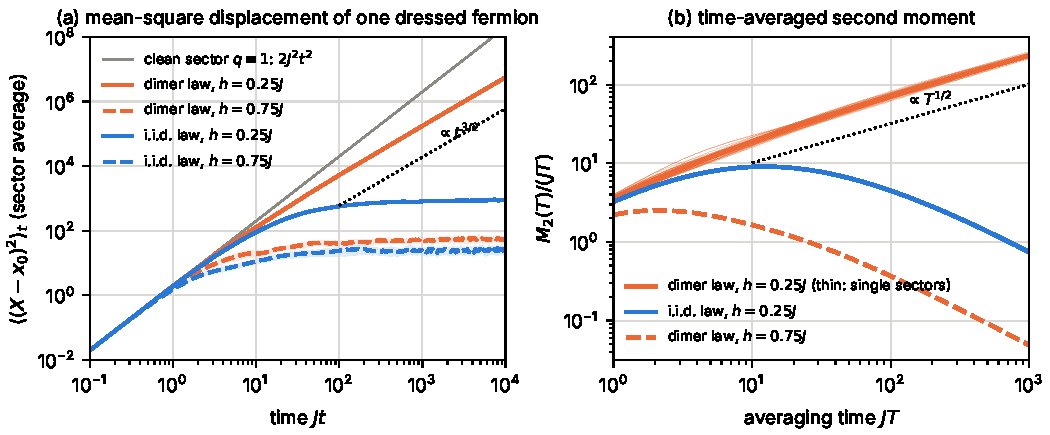
\includegraphics[width=\textwidth]{figs/dimer.pdf}
\caption{A single dressed fermion in the dimer state $\Psi^x=\cdr^\dagger_x\Omdim$ versus the i.i.d.\ law of
\cite{SKKM2017}, at $h=0.25J$ ($\lambda=0.5$, critical energies present) and $h=0.75J$
($\lambda=1.5$, none), with $J=1$.  The one-body dynamics is computed on $\Z$ (no boundary is reached)
and averaged over $64$ sectors.  (a) Sector-averaged mean-square
displacement $\langle(X-x)^2\rangle_t=D^{(N)}_2(t;x)$ in the thermodynamic limit, with bands of $\pm2$
standard errors.  The grey line is the clean sector $q\equiv1$ ($2J^2t^2$, \cref{rem:gaussproj}); the
dotted line has slope $3/2$.  (b) The
time average $\Mom_2(T)/(JT)$ of \cref{thm:dimer}.  Thin lines are the $64$ individual dimer sectors
at $h=0.25J$; each stays bounded below, as \cref{prop:dimerlower} asserts for every configuration, and
their mean grows roughly like $T^{1/2}$ (dotted), consistent with \cref{thm:dimer}(c).  For the
i.i.d.\ law, and for the dimer law at $h=0.75J$, $\Mom_2(T)$ saturates.  Code:
\texttt{code/dimer\_spread.py}; numerical values in \texttt{code/dimer\_spread.out}.}
\label{fig:dimer}
\end{figure}

\begin{remark}[Numerical illustration]\label{rem:dimernumerics}
\Cref{fig:dimer} shows the sector-averaged mean-square displacement of one dressed fermion for the
dimer law and the i.i.d.\ law, at $h=0.25J$ and $h=0.75J$, each averaged over $64$ sectors.  The
one-body dynamics is computed on $\Z$ by Chebyshev propagation on an adaptive window, which contains
every site where the wave function exceeds $10^{-18}$.  So no boundary is ever reached (the largest
window has $3.7\times10^4$ sites), and the data represent the thermodynamic limit of
\cref{thm:dimer}(b).  The propagation agrees with exact diagonalization to $3\times10^{-15}$, and the
norm is conserved to $3\times10^{-12}$.
\begin{itemize}
\item \emph{Dimer law, $h=0.25J$} ($\lambda=\frac12$, critical energies $\pm\lambda$):
$\langle(X-x)^2\rangle_t\approx1.3\times10^2$, $5.3\times10^3$, $1.8\times10^5$ and $5.6\times10^6$ at $Jt=10$,
$10^2$, $10^3$ and $10^4$.  The local exponents over the three decades are $1.62$, $1.52$ and $1.50$, in
line with the $t^{3/2}$ law of \cite{DWP1990} and with the exponent of \cref{thm:dimer}(c).
\item \emph{Saturation.}  For the i.i.d.\ law at $h=0.25J$ the same quantity saturates at
$\approx8.6\times10^2$.  At $h=0.75J$ ($\lambda=1.5$, covered by \cite[Thm.~2.3]{DeBievreGerminet2000},
\cref{rem:dimerstrong}) it saturates at $\approx50$ for the dimer law and at $\approx25$ for the i.i.d.\ law.
\item \emph{Time averages.}  In panel (b), $\Mom_2(T)$ is computed from the same data by the trapezoidal
rule.  On a finite chain this agrees with the exact eigenfunction formula to a relative error of
$10^{-4}$.  For the dimer law at $h=0.25J$, $\Mom_2(T)/(JT)\approx3.6$, $19$, $72$ and $2.3\times10^2$ at
$JT=1$, $10$, $10^2$ and $10^3$.  The smallest value over the $64$ sectors is $3.2$, $16$, $62$ and
$2.1\times10^2$.
\end{itemize}
These numbers illustrate \cref{thm:dimer}; they are not used in any proof.  The check script of
\cref{rem:dimerED} also tests \cref{lem:dimercritical}: the classification (ii) for $13$
values of $\lambda\in(0,3]$, the identities \eqref{eq:dimerrot} to $3\times10^{-15}$, the values
\eqref{eq:dimerangles} (computed independently from the eigenvalues of $D_-(\lambda)$), the commutator
formula (i) on a grid of energies, and the absence of critical energies for the anti-dimer law of
\cref{rem:dimersigns}.  It checks the bound \eqref{eq:dimerTbound} on $120$ random configurations,
alignments, energies and segments; the largest ratio of the two sides is $0.16$.  It verifies
\eqref{eq:quadid} to $10^{-15}$, \eqref{eq:dimerimbid} to $4\times10^{-14}$ ($100$ configurations,
$N=200$), and the Plancherel formula \eqref{eq:plancherel} to $10^{-8}$.  Finally, it checks
\eqref{eq:dimerlower} on a chain of $600$ sites for random, clean and periodic dimer configurations;
there the left side exceeds $c_{\lambda,2}T$ by a factor of at least $10^8$.
\end{remark}

\begin{remark}[Summary: the role of the initial state]\label{rem:dimermessage}
The Hamiltonian, the duality and the gauge-invariant observables are the same throughout this section.
For the $z$-polarized state of \cite{SKKM2017} the charges are i.i.d., and
Theorem~\ref{thm:EC} gives uniform, sector-averaged dynamical localization for every $h\neq0$
(\cref{sec:main}).  For the dimer states, which differ only in the orientation of the even links,
the charges come in neutral pairs.  For $0<2|h|<J$ transport is then at least diffusive in every
sector and superdiffusive on average (\cref{thm:dimer}), and for every $h\neq0$ the infinite-time
average of the CDW imbalance vanishes in the thermodynamic limit (\cref{prop:dimerimbalance}).  In the language of disordered systems, the initial state
selects the statistics of the effective disorder.  Correlations of the dimer type are known to produce
anomalous, superdiffusive transport \cite{DWP1990,JSBS2003}, although the spectrum remains almost surely
pure point \cite{DeBievreGerminet2000} (\cref{rem:dimerstrong}(iii)).  The strictly gauge-invariant sector $q\equiv1$ is not
localized at all (\cref{rem:gaussproj}).  Disorder-free localization is
therefore a joint property of the Hamiltonian and of the sector law induced by the initial state.
\end{remark}
